\chapter{Notacja i niezbędne definicje}\label{preliminaries}

W tej pracy przyjmujemy, że działamy w przestrzeni euklidesowej w skończonym wymiarze $d > 0$.

\begin{definition}
    Niech $x = (x_{1}, \dots, x_{d}) \in \mathbb{R}^{d}$.
    \emph{Normą typu $l_{2}$} nazywamy odwzorowanie $\| \cdot \|: \mathbb{R}^{d} \rightarrow \mathbb{R}$ określone wzorem:
    \begin{equation}
        \|x\|_{2} = \|x\| = \sqrt{ \sum_{i = 1}^{d} x_{i}^{2} }
    \end{equation}
\end{definition}

\noindent
Załóżmy, że mamy dany konkretny problem optymalizacyjny. 

\begin{definition}
    \emph{$\alpha$-aproksymacją} dla problemu optymalizacyjnego nazywamy wielomianowy algorytm, który dla każdej instancji $I$ problemu minimalizacyjnego oblicza rozwiązanie, którego wartość spełnia: 
    \begin{equation}
        A(I) \leq \alpha \cdot OPT
    \end{equation}
    gdzie $A$ jest wartością obliczonego rozwiązania dla instancji $I$, a $OPT$ jest wartością optymalnego rozwiązania tej instancji.
    Zmienną $\alpha$ nazywamy \textit{współczynnikiem aproksymacji}.
    Analogicznie możemy zdefiniować  \emph{$\alpha$-aproksymację} dla problemu maksymalizacyjnego.
    Jest nim wielomianowy algorytm, który dla każdej instancji $I$ spełnia:
    \begin{equation}
        A(I) \geq \frac{1}{\alpha} \cdot OPT
    \end{equation}
    gdzie $A$ i $OPT$ są zdefiniowane tak jak wyżej.
\end{definition}

\begin{definition}
    \emph{Wielomianowym schematem aproksymacji} dla problemu optymalizacyjnego nazywamy rodzinę algorytmów $\{A_{\epsilon}\}$, która dla danego $\epsilon > 0$ zawiera algorytm aproksymacyjny $A_{\epsilon}$ o wspołczynniku aproksymacji równym $(1+\epsilon)$ dla problemu minimalizacyjnego albo $(1-\epsilon)$ dla problemu maksymalizacyjnego.
    Złożoność algorytmu $A_{\epsilon}$ jest wielomianowa ze względu na rozmiar instancji problemu podanej na wejściu $A_{\epsilon}$.
\end{definition}

\noindent
W poprzedniej definicji złożoność algorytmu $A_{\epsilon}$ jest niegraniczona względem $\frac{1}{\epsilon}$.
Oznacza to, że złożoność algorytmu $A_{\epsilon}$ może być wykładniczo zależna od $\frac{1}{\epsilon}$.
W związku z tym wprowadzimy silniejszą definicję 2.3.

\begin{definition}
    \emph{W pełni wielomianowym schematem aproksymacji} jest wielomianowy schemat aproksymacji, dla którego złożoność algorytmu $A_{\epsilon}$  jest wielomianowa od $\frac{1}{\epsilon}$.  
\end{definition}


\begin{definition}
    \emph{Centroidem} dla skończonego zbioru punktów $x_{1}, \dots, x_{k} \in \mathbb{R}^{d}$ nazywamy:
    \begin{equation}
        C = \frac{x_{1} + \dots + x_{k}}{k}
    \end{equation}
\end{definition}

\section{K-means}

Zacznijmy od zdefiniowania problemu, dla którego będziemy analizować konstrukcje coresetów.

\begin{definition}
    \emph{Problem k-means.} Niech $X$ będzie skończonym zbiórem punktów z $\mathbb{R}^{d}$. 
    Dla danego $X$ chcemy znaleźć zbiór $k \in \mathbb{N}$ punktów $Q \subset \mathbb{R}^{d}$, który minimalizuje funkcję $\phi_{X}(Q)$ zdefiniowaną następująco:
    \begin{equation}
        \phi_{X}(Q) = \sum_{x \in X} d(x, Q)^{2} = \sum_{x \in X} \min_{q \in Q} || x - q ||^{2} 
    \end{equation}
\end{definition}

\noindent
Definicja 2.6 zakłada, że działamy w przestrzeni euklidesowej.
Uogólnioną wersję można zdefiniować analogicznie, zamieniając $d$ na odpowiednią funkcję miary w danej przestrzeni.

\begin{figure}[H]
    \centering
    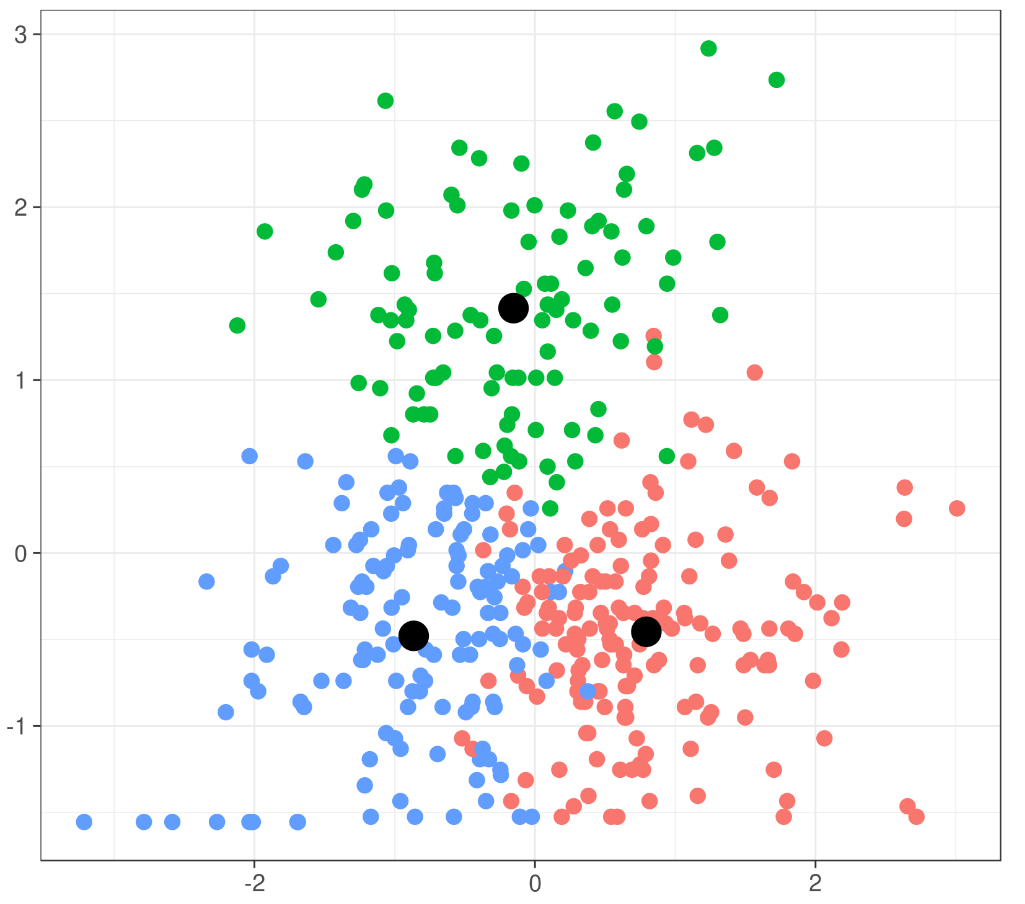
\includegraphics[totalheight=5cm]{cluster.png}
    \caption{Przykład interpretacji problemu $k$-means. Czarne punkty to centroidy, które stanowią zbiór $Q$ optymalizujący funkcję $\phi$.}
\end{figure}

\noindent
Problem $k$-means jest jednym w elementarnych problemów machine learningu.
Używamy go m.in w data miningu, segmentacji obrazu czy klasyfikcji danych. 

\begin{definition}
    \emph{Problem k-means - wersja ważona.} Niech $X_{w}$ będzie skończonym zbiórem punktów z $\mathbb{R}^{d}$ oraz niech $w$ będzie funkcją $w: X_{w} \rightarrow \mathbb{R}_{\ge0}$. 
    Dla danego $X_{w}$ oraz funkcji $w$ chcemy znaleźć zbiór $k \in \mathbb{N}$ punktów $Q \subset \mathbb{R}^{d}$, który minimalizuje funkcję $\phi_{X_{w}}(Q)$ zdefiniowaną następująco:
    \begin{equation}
        \phi_{X_{w}}(Q) = \sum_{x \in X_{w}} w(x) d(x, Q)^{2}
    \end{equation}
\end{definition}

\noindent
Wartość funkcji $\phi$ dla optymalnego rozwiązania oznaczamy $\phi_{opt}^{k}(X)$ lub $OPT$.
W pracy często będziemy korzystać ze stwierdzenia \textit{optymalne rozwiązanie}, które oznacza $k$ elementowy zbiór $C_{opt}$, dla którego wartość funkcji $\phi$ jest zminimalizowana. 
Funkcję $\phi$ w literaturze nazywamy błędem kwantyzacji.

\begin{definition}
    \emph{Klasterem} nazywamy skończony zbioru punktów $x_{1}, \dots, x_{k} \in \mathbb{R}^{d}$, które łączy pewna wspólna cecha.
    W naszym kontekście wspólną cechą bedzie przyporządkowanie do tego samego centroidu.
\end{definition}

\section{Coreset}

To jak definujemy coreset ściśle zależy od problemu, który optymalizujemy.
Zacznijmy od podstawowej definicji coresetu dla problemu $k$-means.

\begin{definition}
    \emph{$(\epsilon, k)$-aproksymacja zbioru centroidów.} 
    Niech $X$ będzie skończonym zbiórem punktów z $\mathbb{R}^{d}$.
    Skończony zbiór $A \subset \mathbb{R}^{d}$ nazywamy $(\epsilon, k)$-aproksymacją zbioru centroidów, gdzie $\epsilon \in (0, 1)$ oraz $k \in \mathbb{N}$, jeżeli istnieje $k$ elementowy podzbiór $C \subseteq A$, dla którego zachodzi:
    \begin{equation}
        |\phi_{X}(C_{opt}) - \phi_{X}(C)| \leq \epsilon\phi_{X}(C_{opt})
    \end{equation}
    gdzie $C_{opt}$ optymalizuje wartość funkcji $\phi$.
\end{definition}

\noindent
Intuicyjnie $(\epsilon, k)$-aproksymację zbioru centroidów możemy rozumieć jako zbiór $A \subset \mathbb{R}^{d}$, który zawiera $k$ elementowy podzbiór $C \subseteq A$ \textit{dobrze} aproksymujący $C_{opt}$.
Definicja 2.9 pojawia się tutaj z dwóch powodów.
Po pierwsze jest ona pewngo rodzaju prekursorem coresetów, a po drugie jest ona konieczna w definicji 2.10.

\begin{definition}
    \emph{Coreset.} Niech $X$ będzie skończonym zbiórem punktów z $\mathbb{R}^{d}$.
    Skończony zbiór $C \subset \mathbb{R}^{d}$ nazywamy $(\epsilon, k)$ coresetem, gdzie $\epsilon \in (0, 1)$, jeżeli dla dowolnego $k \in \mathbb{N}$ elementowego zbioru $Q \subset \mathbb{R}^{d}$ zachodzi:
    \begin{equation}
        |\phi_{X}(Q) - \phi_{C}(Q)| \leq \epsilon\phi_{X}(Q)
    \end{equation}
\end{definition}

\noindent
Zauważmy, że taka definicja daje nam bardzo moce gwarancje teoretyczne.
Wartość funkcji $\phi_{C}(Q)$ aproksymuje $\phi_{X}(Q)$ ze współczynnikiem aproksymacji równym $(1+\epsilon)$ dla dowolnego zbioru $k$ kandydatów $Q$ na rozwiązanie problemu $k$-means.
Jest to na tyle istotne, że w literaturze odróżnimy taką wersję nazywając ją \textit{strong coresetem}.
Definicja 2.10 jest wariantem ciągłym, czyli punkty należące do coresetu są dowolnymi punktami przestrzeni, w szczególności nie muszą należeć do zbioru $X$.
W praktyce stosuje się wariant dyskretny, który zakłada, że $C \subseteq X$.

\begin{figure}[H]
    \centering
    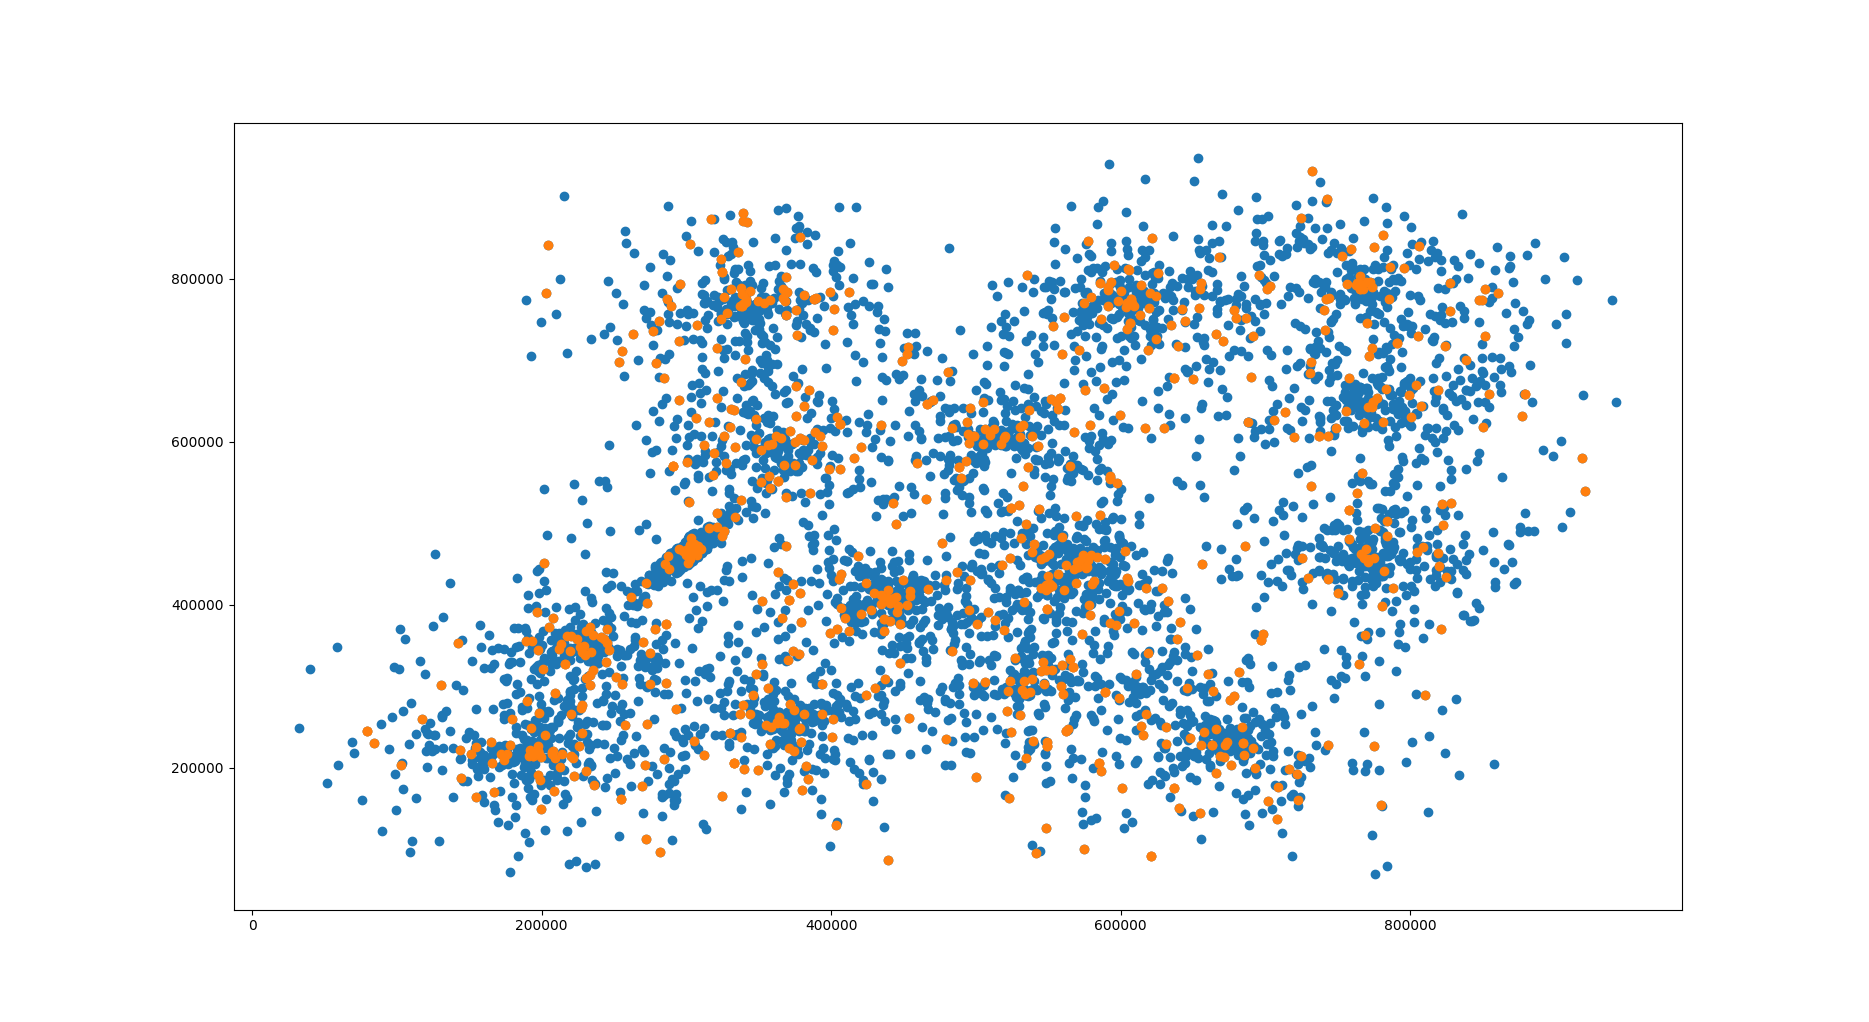
\includegraphics[totalheight=7cm]{coreset.png}
    \caption{Pomarańczowe punkty tworzą coreset dla zbioru niebieskich punktów. 
    Parametry: $k=15$, $\epsilon = 0.1$, $n = 15000$.}
\end{figure}

\begin{definition}
    \emph{Coreset - wersja ważona.} Niech $X_{w}$ będzie skończonym zbiórem punktów z $\mathbb{R}^{d}$ oraz niech $w$ będzie funkcją $w_{x}: X_{w} \rightarrow \mathbb{R}_{\ge0}$.
    Skończony zbiór $C_{w} \subset \mathbb{R}^{d}$ wraz z funkcją $w_{c}: C_{w} \rightarrow \mathbb{R}_{\ge0}$ nazywamy $(\epsilon, k)$ coresetem, gdzie $\epsilon \in (0, 1)$, jeżeli dla dowolnego $k \in \mathbb{N}$ elementowego zbioru $Q \subset \mathbb{R}^{d}$ zachodzi:
    \begin{equation}
        |\phi_{X_{w}}(Q) - \phi_{C_{w}}(Q)| \leq \epsilon\phi_{X_{w}}(Q)
    \end{equation}
\end{definition}

\noindent
Tak samo jak w problemie $k$-means, coreset może być zdefiniowany w wariancie ważonym.
Oznacza to, że dla zbióru $C$ z definicji 2.10  musimy zdefinujować funkcję wag $w_{c}: C \rightarrow \mathbb{R}_{\ge0}$.
Nierówność pozostaje bez zmian, ponieważ funkcja $\phi$ uwzględnia $C_{w}$ oraz $X_{w}$ będące zbiorami ważonymi.

\begin{definition}
    \emph{Coreset - weak (w wariancie dyskretnym).} Niech $X$ będzie skończonym zbiorem punktów z $\mathbb{R}^{d}$.
    Niech $C \subseteq X$ oraz $A$ jest $(\epsilon, k)$-aproksymacją zbioru centroidów dla zbioru $X$, gdzie $\epsilon \in (0, 1)$.
    Jeżeli, dla dowolnego $k \in \mathbb{N}$ elementowego podzbióru $Q \subseteq A$ zachodzi:
    \begin{equation}
        |\phi_{X}(Q) - \phi_{C}(Q)| \leq \epsilon\phi_{X}(Q)
    \end{equation}
    to parę $(C, A)$ nazwiemy słabym coresetem.
\end{definition}

\noindent
\textit{Słabość} definicji 2.12 wynika z konieczności budowy zbioru $A$.
Intuicyjnie zbiór $A$ pomaga coresetowi w zachowaniu odpowiedniego współczynnika aproksymacji, ponieważ w zbiorze $A$ istnieje \textit{dobry} kandydat na rozwiązanie.
W pracy korzystamy wyłącznie z definicji 2.10 oraz 2.11.
Z uwagi na to, że nasza praca ma charakter przeglądowy zdefiniowaliśmy wszystkie możliwe warianty coresetów.